\documentclass[handout,compress]{beamer}
\usepackage[utf8]{inputenc}

\title{Multivariable Calculus (CS+AI)}
\author{Aron Hardeman}
\date{\today}



%\iffalse
\usetheme{Madrid}
%\usecolortheme{whale}
\setbeamercolor{palette primary}{bg=olive!70!black}
\setbeamercolor{palette secondary}{bg=olive!90!black}
\setbeamercolor{palette tertiary}{bg=olive!50!black}
\useoutertheme[subsection=false]{miniframes}
\setbeamertemplate{section in toc shaded}[default][44]
\setbeamertemplate{subsection in toc shaded}[default][44]
%\fi
% a terrible color scheme BELOW, normal color scheme ABOVE
\iffalse
\usetheme{Madrid}
%\usecolortheme{whale}
\setbeamercolor{palette primary}{bg=violet,fg=yellow!80!white}
\setbeamercolor{palette secondary}{bg=cyan!90!violet,fg=lime!10!white}
\setbeamercolor{palette tertiary}{bg=yellow!10!orange,fg=green!10!white}
\setbeamercolor{background canvas}{bg=yellow!80!cyan}
\useoutertheme[subsection=false]{miniframes}
\setbeamertemplate{section in toc shaded}[default][44]
\setbeamertemplate{subsection in toc shaded}[default][44]
\fi


\newenvironment{theorybox}[1]
{
    \begin{tcolorbox}[colback=yellow!50,colframe=green!25!red,title={#1}]
}
{
\end{tcolorbox}
}
\newcommand{\vabla}{\vec{\nabla}}
\newcommand{\lenvec}[1]{|\vec{#1}|}
\newcommand{\red}[1]{\textcolor{red}{#1}}
\newcommand{\gray}[1]{\textcolor{gray!70!white}{#1}}
\newcommand{\blue}[1]{\textcolor{blue}{#1}}
\newcommand{\violet}[1]{\textcolor{violet}{#1}}
\newcommand{\teal}[1]{\textcolor{teal}{#1}}
\newcommand{\yellow}[1]{\textcolor{orange}{#1}}

\usepackage[utf8]{inputenc}
\usepackage{amssymb,amsmath}
\usepackage{tikz}
\usepackage{tikz-qtree}
\usepackage{color}
\usepackage{fancyhdr}
\usepackage{lplfitch}
\usepackage{fancyhdr}
\usepackage{graphicx}
\usepackage[listings,theorems]{tcolorbox}
\usepackage{float}
\usepackage{natbib}
\usepackage{stmaryrd}
\usepackage{relsize}
\usepackage{ulem}
\usepackage{cancel}
\usepackage{tensor}
\usepackage{pgfplots}
\usepgfplotslibrary{polar}
\usepgfplotslibrary{fillbetween}
\usetikzlibrary{quotes,angles}
\usetikzlibrary{babel}
\usetikzlibrary{shapes,positioning,intersections}
\usepackage{verbatim}
\pgfplotsset{width=8cm,compat=1.9}

\DeclareMathOperator{\atantwo}{atan2}
\DeclareMathOperator{\Arg}{Arg}


\begin{document}

\maketitle

\section{Derivatives}
\subsection{Partial derivatives}
\tableofcontents[currentsection,currentsubsection]

\begin{frame}
\frametitle{Derivatives}

We already know how to compute the derivative of a function of one variable, e.g., for $f(x)=\sin(x^2)$ we get:
\[\frac{d f}{dx}=2x\cos(x^2) \qquad \frac{d^2 f}{dx^2}=2\cos(x^2)-4x^2\sin(x^2)\]

If we have a function of more than one variable, say $g(x,y,z)=x^5y+3e^z$, then we can compute three \textit{partial derivatives}, one with respect to each input variable.

The partial derivative of $g$ with respect to $x$ is denoted $\frac{\partial g}{\partial x}$ or $g_x$.

The partial derivative of $g$ with respect to $y$ is denoted $\frac{\partial g}{\partial y}$ or $g_y$.

The partial derivative of $g$ with respect to $z$ is denoted $\frac{\partial g}{\partial z}$ or $g_z$.

Notice that we use a ``curly d'' ($\partial$) for partial derivatives.

\end{frame}

\begin{frame}
\frametitle{Computing partial derivatives}

To compute partial derivatives, we use this rule: \textbf{in order to compute the partial derivative with respect to one variable (say $x$), we use the regular derivative rules that we already know, while regarding the other variables ($y$ and $z$) as \textit{constants}.}

\vspace{3mm}Take $g(x,y,z)=x^5y+3e^z$:
\[g_x = 5x^4y\qquad g_y=x^5\qquad g_z=3e^z\]
For example, when we compute $g_x$, we see that the $3e^z$ term vanishes (since we regard $z$ as a constant, $3e^z$ is also constant, and the derivative of a constant is $0$). And the derivative of the term $x^5y$ is just $5x^4y$, since $y$ is regarded as constant.

\end{frame}

\begin{frame}
\frametitle{Higher order partial derivatives}

Of course, we can also take the derivative of the derivative, and compute higher order partial derivatives in that way. Take for example $f(x,y,z)=xe^y\sin(z^2)$,
\[f_x = e^y\sin(z^2)\qquad f_y=xe^y\sin(z^2)\qquad f_z=2xe^y z\cos(z^2)\]

There are nine second order partial derivatives ($f_{xy}=(f_x)_y$):
{\footnotesize\begin{align*}
    f_{xx} = 0 \qquad&& \textcolor{blue}{f_{yx} = e^y\sin(z^2)} \qquad&& \textcolor{red}{f_{zx} = 2e^y z\cos(z^2)}\\
    \textcolor{blue}{f_{xy} = e^y\sin(z^2)} \qquad&& f_{yy} = xe^y\sin(z^2)\qquad&& \textcolor{teal}{f_{zy} =  2xe^y z\cos(z^2)} \\
    \textcolor{red}{f_{xz} = 2e^y z\cos(z^2)}\qquad&& \textcolor{teal}{f_{yz} = 2xe^y z\cos(z^2)} \qquad&& f_{zz} = 2xe^y\left[\cos(z^2)-2z^2\sin(z^2)\right]
\end{align*}}
We observe that in the end, the order of differentiation did not matter: $f_{xy}=f_{yx}$, and $f_{xz}=f_{zx}$, and $f_{yz}=f_{zy}$. In fact, this is always the case for any function\footnote{As long as the function has continuous second order partial derivatives}. \textit{(Clairaut's theorem)}.

\end{frame}



    \subsection{The gradient \& directional derivative}
\tableofcontents[currentsection,currentsubsection]
\begin{frame}
\frametitle{The gradient vector}

The gradient is the vector of first-order partial derivatives of a function.

For functions of two or three variables, the gradient is
\[\vec{\nabla} f(x,y) =
\begin{bmatrix}
\frac{\partial}{\partial x} f(x,y)\\
\frac{\partial}{\partial y} f(x,y)\\
\end{bmatrix}
\qquad
\vec{\nabla} g(x,y,z) =
\begin{bmatrix}
\frac{\partial}{\partial x} g(x,y,z)\\
\frac{\partial}{\partial y} g(x,y,z)\\
\frac{\partial}{\partial z} g(x,y,z)\\
\end{bmatrix}
\]


The gradient of $f$ can also be written as $\text{grad } f$ or $\nabla f$, but in these slides we use $\vec{\nabla} f$ in order to accentuate the vectorial nature of the gradient.

The gradient is important, because the directional derivative of a function at a point is maximal when you go in the direction of the gradient. \textbf{So, the gradient gives the direction of steepest increase of a function.}

\end{frame}


\begin{frame}
\frametitle{The directional derivative}

When you have a function $f$ of more than one input variable, say $f(x,y)$, you might wonder what the rate of change \textit{in a particular direction} is. This is the \textbf{directional derivative}.
    \begin{theorybox}{Directional derivative}
    The directional derivative of $f(x,y)$ in the direction of a \textbf{UNIT} vector $\hat{u}=\begin{bmatrix}a\\b\end{bmatrix}$ is
    \[D_{\hat{u}}f(x,y)=f_x(x,y)a+f_y(x,y)b=\vabla f(x,y)\cdot\hat{u}\]

    Similarly, in three dimensions, the directional derivative of $f(x,y,z)$ in the direction of a \textbf{\textcolor{red}{UNIT}} vector $\hat{u}=[a~~b~~c]^T$ is given by
    \[D_{\hat{u}}f(x,y,z)=f_x(x,y,z)a+f_y(x,y,z)b+f_z(x,y,z)c=\vabla f(x,y,z)\cdot\hat{u}\]
    
\end{theorybox}
\end{frame}

\begin{frame}{Directional derivative: example}
\footnotesize
    \begin{itemize}
        \item \textbf{Question:} calculate the directional derivative of $f(x,y)=4x^2+xe^{x+2y}-ye^{2x+y}+42$ in the direction of the vector $\vec{v}=\begin{bmatrix}-4\\3\end{bmatrix}$ at the point $(5,6)$.
        \item \textbf{Step 1:} observe that $\vec{v}$ is \textbf{not a unit vector}. We have to convert it into a unit vector by dividing it by its length $\lenvec{v}=\sqrt{(-4)^2+3^2}=5$.
        \[\hat{v}=\frac{\vec{v}}{\lenvec{v}}=\begin{bmatrix}\textcolor{red}{-4/5}\\\textcolor{blue}{3/5}\end{bmatrix}\]
        \item \textbf{Step 2:} calculate the partial derivatives:
        \begin{align*}
            f_x(x,y)&=8x+(1+x)e^{x+2y}-2ye^{2x+y}\qquad&f_x(5,6)&=40+6e^{17}-12e^{16}\\
            f_y(x,y)&=2xe^{x+2y}-(1+y)e^{2x+y} &f_y(5,6)&=10e^{17}-7e^{16}
        \end{align*}
        \item \textbf{Step 3:} the directional derivative is: (do not forget to use the \textit{unit} vector!)
        \begin{align*}D_{\hat{v}}f(5,6)&=\textcolor{red}{-\frac{4}{5}}f_x(5,6)+\textcolor{blue}{\frac{3}{5}}f_y(5,6)\\
        &=\textcolor{red}{-\frac{4}{5}}(40+6e^{17}-12e^{16})+\textcolor{blue}{\frac{3}{5}}(10e^{17}-7e^{16})=\boxed{-32+\frac{27}{5}e^{16}+\frac{6}{5}e^{17}}
        \end{align*}
    \end{itemize}
\end{frame}


\subsection{Tangent planes}
\tableofcontents[currentsection,currentsubsection]

\begin{frame}{Tangent planes}
    \begin{theorybox}{Tangent planes}
        \textbf{Case 1:} When you have a function $f(x,y)$ and consider the surface given by all points $(x,y,f(x,y))$, then the tangent plane to the surface at $(a,b,f(a,b))$ is given by \[\boxed{z=f(a,b)+f_x(a,b)(x-a)+f_y(a,b)(y-b)}\]

        \textbf{Case 2:} When you have a function $f(x,y,z)$ and consider the surface given by all points for which $f(x,y,z)=K$ (for some $K$), then the tangent plane to the surface at $(a,b,c)$ is given by
        \[\boxed{f_x(a,b,c)(x-a)+f_y(a,b,c)(y-b)+f_z(a,b,c)(z-c)=0}\]
    \end{theorybox}
\end{frame}

\begin{frame}{Tangent planes: example}
    \begin{itemize}
        \item
            \textbf{Question:} Given the function $z=f(x,y)=3xy+e^{xy^2+3}$, find the tangent plane to this surface at the point $(-3,1)$.
        \item \textbf{Step 1:} We decide to use "case 1" from the previous slide. Calculate the partial derivatives:
            \[f_x(x,y)=3y+y^2e^{xy^2+3}  \qquad  f_y(x,y)=3x+2xye^{xy^2+3}\]
            \[f_x(-3,1)=4 \qquad f_y(-3,1)=-15\]
        \item \textbf{Step 2:}
            The tangent plane is thus
            \[\boxed{z=-8+4(x+3)-15(y-1)}\]
        \item \gray{Step 3: rewrite nicely:}
            \[{\gray{4x-15y-z=-19}}\]
    \end{itemize}
\end{frame}

\begin{frame}{Tangent planes: another example}
    \begin{itemize}
        \item
            \textbf{Question:} find the tangent plane to the surface given by $x^2y^3+3x^3+x^2y+xyz^2+yz^2=xy$ at the point $(1,-1,1)$.
        \item \textbf{Step 1:}  We recognize that we can define $f(x,y,z)=x^2y^3+3x^3+x^2y+xyz^2+yz^2-xy$, and then the surface is just $f(x,y,z)=0$. So we decide to use "case 2" from the schema.
        \item \textbf{Step 2:} calculate the partial derivatives:
            \begin{align*}
                f_x(x,y,z)&=2xy^3+9x^2+2xy+yz^2-y & f_x(1,-1,1)=5\\
                f_y(x,y,z)&=3x^2y^2+x^2+xz^2+z^2-x & f_y(1,-1,1)=5\\
                f_z(x,y,z)&=2xyz+2yz & f_z(1,-1,1)=-4
            \end{align*}
        \item \textbf{Step 3:} The tangent plane is thus (see "case 2"):
            \[\boxed{5(x-1)+5(y+1)-4(z-1)=0}\]

    \end{itemize}
\end{frame}

\section{Double integrals}
\subsection{In Cartesian coordinates ($x,y$)}
\tableofcontents[currentsection,currentsubsection]
\begin{frame}{Double integrals (intuition)}
    Sometimes we need to take an integral over a integral.
    This is useful for example when calculating the volume of a 3D body.
    \begin{itemize}
        \item \textbf{Question:} calculate the volume of the 3D body between $z=f(x,y)=(2x+3)e^y$ and the $xy$-plane, when the bounds of $x$ and $y$ are the rectangle $-1\leq x\leq1$ and $0\leq y\leq2$.
        \item \textbf{Intuition:} the volume consists of a large number of very small ``boxes'' (3D-rectangles). The volume of one such ``box" is $\text{length}\cdot\text{width}\cdot\text{height}=dx\cdot dy\cdot(2x+3)e^y$. The total volume of the 3D body must be the sum of all these little boxes, i.e., an integral:
            \[V_{\text{tot}}=\int_{0}^{2}\int_{-1}^{1}(2x+3)e^y dxdy=\int_{-1}^{1}\int_{0}^{2}(2x+3)e^y dydx\]
        The next slides cover how to compute such a double integral.
    \item    \textbf{Note:} in the case of a rectangle, the order of integration does not matter (that's why the two double integals above are equivalent).
    \end{itemize}
\end{frame}

\begin{frame}{Computing normal double integrals (1/2)}
    \begin{itemize}
        \item \textbf{Question:} calculate the volume of the 3D body between $z=f(x,y)=(2x+3)e^y$ and the $xy$-plane, when the bounds of $x$ and $y$ are the rectangle $-1\leq x\leq1$ and $0\leq y\leq2$.
        \item We need to compute the double integral\footnote{The reverse order would also work:
            $V_{\text{tot}}=\int_{-1}^{1}\red{\int_{0}^{2}(2x+3)e^y dy}dx$}
            \[V_{\text{tot}}=\int_{0}^{2}\red{\int_{-1}^{1}(2x+3)e^y dx}dy\]
        \item \textbf{Plan of attack:} work from the inside-out. So, we start solving the inner integral: $\red{\int_{-1}^{1}(2x+3)e^y dx}$. \textbf{Important:} this is an integral in the ``$x$-world", because of the $dx$. It means that $x$ changes, whereas we can treat $y$ as a constant when computing the integral. So:
            \[\red{\int_{-1}^{1}(2x+3)e^y dx}=e^y\int_{-1}^1(2x+3)dx=e^y\left[x^2+3x\right]_{-1}^1=6e^y\]
    \end{itemize}
\end{frame}

\begin{frame}{Computing normal double integrals (2/2)}
    \begin{itemize}
        \item \textbf{Question:} calculate the volume of the 3D body between $z=f(x,y)=(2x+3)e^y$ and the $xy$-plane, when the bounds of $x$ and $y$ are the rectangle $-1\leq x\leq1$ and $0\leq y\leq2$.
            \[V_{\text{tot}}=\int_{0}^{2}\blue{\int_{-1}^{1}(2x+3)e^y dx}dy\]
        \item We found:
            \[\blue{\int_{-1}^{1}(2x+3)e^y dx}=\red{6e^y}\]
        \item We substitute this into the original double integral:
            \[V_{\text{tot}}=\int_{0}^{2}\red{6e^y}dy=6\left[e^y\right]_0^2=6e^2-6\]
        \item \textbf{Conclusion:} the volume of the 3D body is $\boxed{V_{\text{tot}}=6e^2-6}$.
    \end{itemize}
\end{frame}


\begin{frame}{Another simple double integral}
    \begin{itemize}
        \item \textbf{Question:} calculate the volume of the 3D body between $z=f(x,y)=\frac{x^3}{y}$ and the $xy$-plane, when the bounds of $x$ and $y$ are the rectangle $3\leq x\leq5$ and $2\leq y\leq4$.
        \item We want to solve the integral
            \[\int_2^4\int_3^5\frac{x^3}{y}dxdy\]
            We start with solving the inner integral, where $x$ changes and $y$ is constant:
            \[\int_3^5\frac{x^3}{y}dx=\frac{1}{y}\int_3^5x^3dx=\frac{1}{4y}\left[x^4\right]_3^5=\frac{136}{y}\]
            Now we calculate the full double integral: the volume is
            \[\int_2^4\int_3^5\frac{x^3}{y}dxdy=\int_2^4\frac{136}{y}dy=136\left[\ln y\right]_2^4=\boxed{136\ln2}\]
    \end{itemize}
\end{frame}

\begin{frame}{Double integrals over general regions (1/2)}
         \textbf{Question:} calculate the volume of the 3D body between the paraboloid $z=x^2+y^2$ and the $xy$-plane, above the region $D$ enclosed by the parabola $y=3x^2$ and the line $y=x+2$.

            \begin{minipage}{0.4\textwidth}
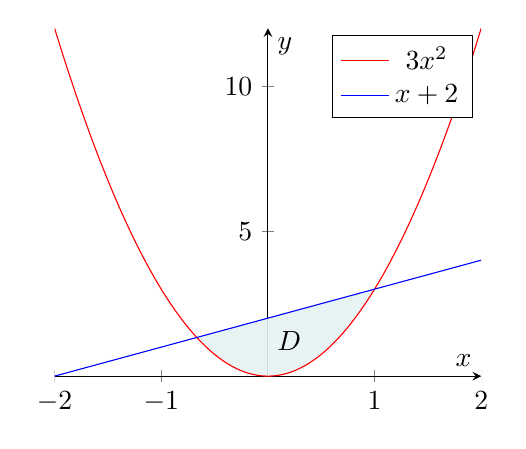
\begin{tikzpicture}
\begin{axis}[
    xlabel = \(x\),
    ylabel = {\(y\)},
    axis lines=middle,
    height=6cm,
    width=7cm,
]
\addplot [
    domain=-2:2, 
    samples=100, 
    color=red,
    name path=f,
]
{3*x^2};
    \addlegendentry{\(3x^2\)}
\addplot [
    domain=-2:2, 
    samples=100, 
    color=blue,
    name path=g,
    ]
    {x+2};
    \addlegendentry{\(x+2\)}

    \addplot[teal!10, opacity=0.9] fill between[of=f and g, soft clip={domain=-0.667:1}];
\node at (axis cs:0.2,1.2) {$D$};
\end{axis}
\end{tikzpicture}
            \end{minipage}\hspace{1.5cm}
            \begin{minipage}{0.45\textwidth}

                Solving the equation $3x^2=x+2$ gives the endpoints $x=-\frac{2}{3}$ and $x=1$, so we get \[V=\iint_{D}(x^2+y^2)dA\]\[\boxed{V=\int_{-2/3}^{1}\int_{3x^2}^{x+2}(x^2+y^2)dydx}\]
To be computed in the next slide.
            \end{minipage}

\end{frame}

\begin{frame}{Double integrals over general regions (2/2)}
\small
         We calculate the integral from the previous slide to find the volume:
         \begin{align*}
             V&=\int_{-2/3}^{1}\int_{3x^2}^{x+2}(x^2+y^2)dydx=\int_{-2/3}^{1}\left[x^2y+\frac{y^3}{3}\right]_{y=3x^2}^{y=x+2}dx\\
              &=\int_{-2/3}^{1}\left[x^2(x+2)+\frac{1}{3}(x+2)^3-x^2\cdot3x^2-\frac{1}{3}(3x^2)^3\right]dx\\
              &=\int_{-2/3}^{1}\left[x^3+2x^2+\frac{1}{3}\left(x^3+6x^2+12x+8\right)-3x^4-9x^6\right]dx\\
              &=\int_{-2/3}^{1}\left(-9x^6-3x^4+\frac{4}{3}x^3+4x^2+4x+\frac{8}{3}\right)dx\\
              &=\left[-\frac{9}{7}x^7-\frac{3}{5}x^5+\frac{1}{3}x^4+\frac{4}{3}x^3+2x^2+\frac{8}{3}x\right]_{-2/3}^{1} =\boxed{ \frac{3125}{567}}
         \end{align*}
         So the volume is $\frac{3125}{567}$. \textbf{Note:} in this case, the order of integration matters. We have to first integrate w.r.t. $y$ and then $x$. (Try the other way, it's very hard.)
\end{frame}

\subsection{In polar coordinates ($r,\theta$)}
\tableofcontents[currentsection,currentsubsection]
\begin{frame}{Polar coordinates (1/2)}
    Sometimes we need to do integrals using \textbf{polar coordinates}, which look like this:

    \vspace{0.3mm}
    \begin{minipage}{0.6\textwidth}
    \tikzset{every picture/.style={line width=0.75pt}} %set default line width to 0.75pt        

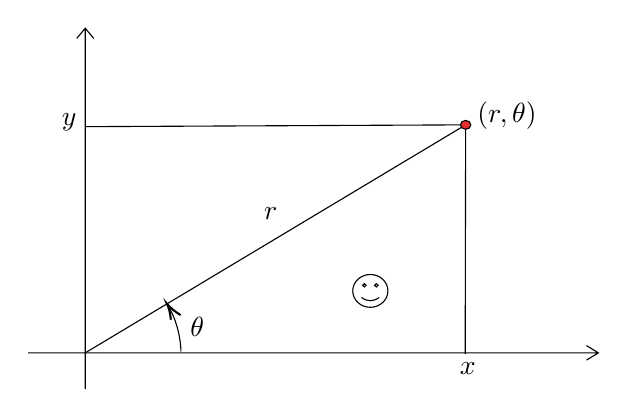
\begin{tikzpicture}[x=0.75pt,y=0.75pt,yscale=-0.7,xscale=0.82]
%uncomment if require: \path (0,285); %set diagram left start at 0, and has height of 285

%Shape: Smiley Face [id:dp830203050540306] 
\draw   (201.67,196.79) .. controls (201.67,190.56) and (206.29,185.5) .. (212,185.5) .. controls (217.71,185.5) and (222.33,190.56) .. (222.33,196.79) .. controls (222.33,203.03) and (217.71,208.08) .. (212,208.08) .. controls (206.29,208.08) and (201.67,203.03) .. (201.67,196.79) -- cycle ; \draw   (207.45,192.95) .. controls (207.45,192.33) and (207.92,191.82) .. (208.49,191.82) .. controls (209.06,191.82) and (209.52,192.33) .. (209.52,192.95) .. controls (209.52,193.58) and (209.06,194.08) .. (208.49,194.08) .. controls (207.92,194.08) and (207.45,193.58) .. (207.45,192.95) -- cycle ; \draw   (214.48,192.95) .. controls (214.48,192.33) and (214.94,191.82) .. (215.51,191.82) .. controls (216.08,191.82) and (216.55,192.33) .. (216.55,192.95) .. controls (216.55,193.58) and (216.08,194.08) .. (215.51,194.08) .. controls (214.94,194.08) and (214.48,193.58) .. (214.48,192.95) -- cycle ; \draw   (206.83,201.31) .. controls (210.28,204.32) and (213.72,204.32) .. (217.17,201.31) ;
%Shape: Axis 2D [id:dp26103124522186905] 
\draw  (11,239.43) -- (346,239.43)(44.5,16) -- (44.5,264.25) (339,234.43) -- (346,239.43) -- (339,244.43) (39.5,23) -- (44.5,16) -- (49.5,23)  ;
%Straight Lines [id:da3997877631677582] 
\draw    (268,82.5) -- (267.75,240.13) ;
%Straight Lines [id:da143433628895133] 
\draw    (268,82.5) -- (44.5,239.43) ;
%Curve Lines [id:da0981281691186493] 
\draw    (100.71,238.5) .. controls (100.71,233.28) and (99.44,218.76) .. (92.82,206.27) ;
\draw [shift={(92.38,205.46)}, rotate = 61.07] [color={rgb, 255:red, 0; green, 0; blue, 0 }  ][line width=0.75]    (10.93,-3.29) .. controls (6.95,-1.4) and (3.31,-0.3) .. (0,0) .. controls (3.31,0.3) and (6.95,1.4) .. (10.93,3.29)   ;
%Straight Lines [id:da7865700687572084] 
\draw    (268,82.5) -- (44.67,83.75) ;
%Shape: Circle [id:dp17179590489530172] 
\draw  [fill={rgb, 255:red, 229; green, 47; blue, 47 }  ,fill opacity=1 ] (264.96,82.5) .. controls (264.96,80.82) and (266.32,79.46) .. (268,79.46) .. controls (269.68,79.46) and (271.04,80.82) .. (271.04,82.5) .. controls (271.04,84.18) and (269.68,85.54) .. (268,85.54) .. controls (266.32,85.54) and (264.96,84.18) .. (264.96,82.5) -- cycle ;

% Text Node
\draw (263,244.65) node [anchor=north west][inner sep=0.75pt]    {$x$};
% Text Node
\draw (29.17,72.65) node [anchor=north west][inner sep=0.75pt]    {$y$};
% Text Node
\draw (104.67,212.98) node [anchor=north west][inner sep=0.75pt]    {$\theta $};
% Text Node
\draw (148,137.65) node [anchor=north west][inner sep=0.75pt]    {$r$};
% Text Node
\draw (273.33,64.98) node [anchor=north west][inner sep=0.75pt]    {$( r,\theta )$};


\end{tikzpicture}

    \end{minipage}
    \begin{minipage}{0.35\textwidth}
        We see the important equations:
        \[\boxed{x^2+y^2=r^2}\]
        \[\boxed{x=r\cos\theta}\]
        \[\boxed{y=r\sin\theta}\]
    \end{minipage}
\end{frame}

\begin{frame}{Polar coordinates (2/2)}
    Back in normal coordinates, we could just say $dA=dxdy$ (or $dA=dydx$). For example:
    \[D=\{(x,y)~\mid~y\leq x\leq y+2~\land~1\leq y\leq 3\}\]
    \[\iint_D f(x,y) \red{dA} = \int_{1}^{3}\int_{y}^{y+2}f(x,y)\red{dxdy}\]

    For polar regions, we replace $dA$ with $rdrd\theta$ (or $rd\theta dr$). For example:
    \[D=\{(r,\theta)~\mid~1\leq r\leq 2~\land~0\leq\theta\leq2\pi\}\]
    \[\iint_D f(r,\theta) \red{dA} = \int_{0}^{2\pi}\int_{1}^{2}f(r,\theta)\red{rdrd\theta}\]
    \red{\textbf{IMPORTANT: it is $dA=r\cdot drd\theta$, NOT $dA=drd\theta$.}}
\end{frame}


\begin{frame}{A ``polar" integral}
\footnotesize
    \begin{itemize}
        \item \textbf{Question:} calculate the volume of the solid body bounded by the function $z=f(x,y)=x^4+2x^2y^2+y^4$ and the $xy$-plane above the circular region in the $xy$-plane given in the plot:

            \begin{minipage}{0.35\textwidth}
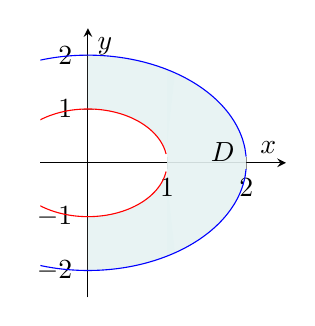
\begin{tikzpicture}
\begin{axis}[
    xlabel = \(x\),
    ylabel = {\(y\)},
    axis lines=middle,
    height=5cm,
    width=4.7cm,
    xmin=-0.6,xmax=2.5,
    ymin=-2.5,ymax=2.5,
    ytick distance=1,
]
\addplot [
    domain=-1:3.5, 
    samples=300, 
    color=red,
    name path=f,
]
    {sqrt(1-x^2)};
\addplot [
    domain=-1:3, 
    samples=300, 
    color=blue,
    name path=h,
]
    {sqrt(4-x^2)};
\addplot [
    domain=-1:3.5, 
    samples=300, 
    color=red,
    name path=g,
    ]
    {-sqrt(1-x^2)};
\addplot [
    domain=-1:2.5, 
    samples=300, 
    color=blue,
    name path=i,
    ]
    {-sqrt(4-x^2)};

\node at (axis cs:1.7,0.2) {$D$};
    \addplot[teal!10, opacity=0.9] fill between[of=f and h, soft clip={domain=0:1.1}];
    \addplot[teal!10, opacity=0.9] fill between[of=h and i, soft clip={domain=1:3}];
    \addplot[teal!10, opacity=0.9] fill between[of=g and i, soft clip={domain=0:1.1}];
\end{axis}
\end{tikzpicture}
            \end{minipage}\begin{minipage}{0.6\textwidth}
                    \item \textbf{Step 1:} we can write the region of the plot as
                        \[D=\{(r,\theta)~\mid~ 1\leq r\leq2 ~\land~ -\pi/2\leq\theta\leq\pi/2\}\]
                    \item \textbf{Step 2:} we have \[f(x,y)=x^4+2x^2y^2+y^4=(x^2+y^2)^2\] Using the identity $x^2+y^2=r^2$, we see that this is equal to $(r^2)^2=r^4$.
            \end{minipage}
                    \item \textbf{Step 3:} set up the integral and solve it:
                        \[V=\int_{-\pi/2}^{\pi/2}\int_1^2 r^4 rdrd\theta=\int_{-\pi/2}^{\pi/2}d\theta\int_1^2 r^5 dr=\pi\left[\frac{1}{6}r^6\right]_1^2=\boxed{\frac{21}{2}\pi}\]
                        So the volume is $\frac{21}{2}\pi$.
    \end{itemize}
\end{frame}

%\begin{frame}{Nasty little question}
%\footnotesize
%    \begin{itemize}
%        \item \textbf{Question:} calculate the volume of the solid body bounded by the function $z=f(x,y)=y\sqrt{x^2+y^2}$ and the $xy$-plane above the shaded region in the $xy$-plane given in the plot (note: only consider $y\geq0$):
%
%            \begin{minipage}{0.45\textwidth}
%\begin{tikzpicture}
%\begin{axis}[
%    xlabel = \(x\),
%    ylabel = {\(y\)},
%    axis lines=middle,
%    height=5cm,
%    width=6.4cm,
%    xmin=-3,ymin=-3,
%    xmax=7,ymax=4,
%]
%    \addplot[domain=0:pi,samples=100,color=red,data cs=polarrad, name path = f] { 3+2*cos(deg(x))};
%    \addplot[domain=0:pi,samples=100,color=violet,data cs=polarrad,name path=g] { 2};
%    \addplot[teal!10, opacity=0.9] fill between[of=g and f, split];
%
%\node at (axis cs:2.8,1.8) {$D$};
%\end{axis}
%\end{tikzpicture}
%            \end{minipage}\begin{minipage}{0.45\textwidth}
%                Here, it is given that the red border is described by the equation \[\sqrt{x^2+y^2}=3+\frac{2x}{\sqrt{x^2+y^2}}\] And the violet border is described by the equation \[x^2+y^2=4\]
%            \end{minipage}
%        \item \textbf{Solution:} next slide
%    \end{itemize}
%\end{frame}


\begin{frame}{Nasty little question (1/4)}
\footnotesize
    \begin{itemize}
        \item \textbf{Question:} calculate the volume of the solid body bounded by the function $z=f(x,y)=y\sqrt{x^2+y^2}$ and the $xy$-plane above the shaded region in the $xy$-plane given in the plot (note: only consider $y\geq0$):

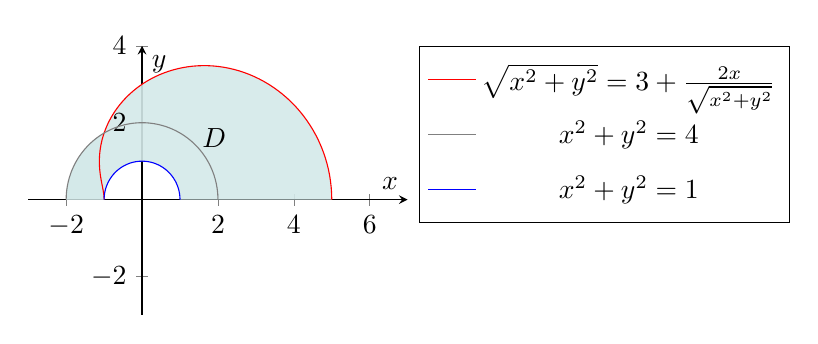
\begin{tikzpicture}
\begin{axis}[
    xlabel = \(x\),
    ylabel = {\(y\)},
    axis lines=middle,
    height=5cm,
    width=6.4cm,
    xmin=-3,ymin=-3,
    xmax=7,ymax=4,
    legend pos=outer north east,
    legend style={minimum height=7mm}
]
    \addplot[domain=0:pi,samples=100,color=red,data cs=polarrad, name path=f] { 3+2*cos(deg(x))};
    \addlegendentry{\(\sqrt{x^2+y^2}=3+\frac{2x}{\sqrt{x^2+y^2}}\)}
    \addplot[domain=0:pi,samples=100,color=gray,data cs=polarrad,name path=g] { 2};
    \addlegendentry{\({x^2+y^2}=4\)}
    \addplot[domain=0:pi,samples=100,color=blue,data cs=polarrad,name path=h] { 1};
    \addlegendentry{\({x^2+y^2}=1\)}
    \addplot[teal!17, opacity=0.9] fill between[of=g and f, split];
    \addplot[teal!17, opacity=0.9] fill between[of=g and h];

\node at (axis cs:1.9,1.6) {$D$};
\end{axis}
\end{tikzpicture}
        \item \textbf{Solution:} next slide
    \end{itemize}
\end{frame}


\begin{frame}{Nasty little question (2/4)}
    \begin{itemize}
        \item Let's first rewrite the equation of the red boundary into polar coordinates (use $x^2+y^2=r^2$ and $x=r\cos\theta$):
            \[\sqrt{x^2+y^2}=3+\frac{2x}{\sqrt{x^2+y^2}} \quad\red{\rightsquigarrow}\quad r=3+2\cos\theta\]
        \item The other boundaries are just half-circles with radii $r=1$ and $r=2$.
    \end{itemize}

    \vspace{3mm}
\begin{minipage}{0.45\textwidth}
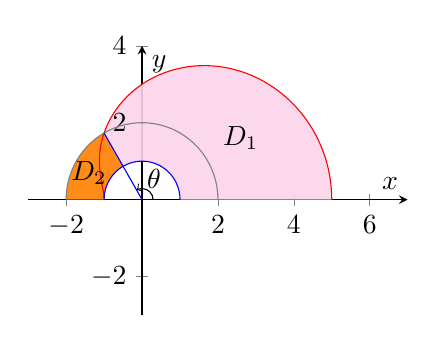
\begin{tikzpicture}
\begin{axis}[
    xlabel = \(x\),
    ylabel = {\(y\)},
    axis lines=middle,
    height=5cm,
    width=6.4cm,
    xmin=-3,ymin=-3,
    xmax=7,ymax=4,
    legend pos=outer north east,
    legend style={minimum height=7mm}
]
    \addplot[domain=0:pi,samples=100,color=red,data cs=polarrad, name path=f] { 3+2*cos(deg(x))};
    \addplot[domain=0:pi,samples=300,color=gray,data cs=polarrad,name path=g] { 2};
    \addplot[domain=0:pi,samples=300,color=blue,data cs=polarrad,name path=h] { 1};
    \addplot[domain=-2:7,samples=300,draw=none,name path=j] { 0};
    \addplot[domain=-1:0,samples=300,color=blue,name path=i] {-sqrt(3)*x};
    \addplot[magenta!17, opacity=0.9] fill between[of=h and f,
    soft clip=i
    ];
    \addplot[orange, opacity=0.9] fill between[of=g and j,soft clip={domain=-2:-1}];
    \addplot[orange, opacity=0.9] fill between[of=h and i,soft clip={domain=-1:-0.5}];

\node at (axis cs:2.6,1.6) {$D_1$};
\node at (axis cs:-1.4,0.7) {$D_2$};
    \coordinate (aaa) at (axis cs:3,0);
    \coordinate (bbb) at (axis cs:0,0);
    \coordinate (ccc) at (axis cs:-1,1.732);
    \pic [draw, ->, "$\theta$", angle eccentricity=2.17, angle radius=1.4mm] {angle = aaa--bbb--ccc};
\end{axis}
\end{tikzpicture}
%\begin{tikzpicture}
%\begin{axis}[
%    xlabel = \(x\),
%    ylabel = {\(y\)},
%    axis lines=middle,
%    height=5cm,
%    width=6.4cm,
%    xmin=-3,ymin=-3,
%    xmax=7,ymax=4,
%]
%    \addplot[domain=0:pi,samples=100,color=red,data cs=polarrad, name path = f] { 3+2*cos(deg(x))};
%    \addplot[domain=0:pi,samples=100,color=violet,data cs=polarrad,name path=g] { 2};
%    \addplot[yellow, opacity=0.9] fill between[of=g and f, split, every odd segment/.style={gray}];
%
%\end{axis}
%\end{tikzpicture}
            \end{minipage}\begin{minipage}{0.45\textwidth}
                We need to split the region; see the picture.\footnote{There are also other ways to split} The angle $\theta$ as in the picture occurs when \[2=3+2\cos\theta\quad\Rightarrow\quad\cos\theta=-\frac{1}{2}\]
                So we split the integral at $\theta=\frac{2}{3}\pi$.
                
            \end{minipage}
\end{frame}




\begin{frame}{Nasty little question (3/4)}
    \footnotesize
                In the previous slide, we calculated that the ``split angle'' is $\theta=\frac{2\pi}{3}$.  

            We can write the region of integration as $D=D_1\cup D_2$ (with $D_{1,2}$ as in the picture on previous slide, note that these regions do not overlap except at the boundary):
            \begin{align*}D &=\{(r,\theta) \mid 0\leq\theta\leq\frac{2\pi}{3} \land 1\leq r\leq 3+2\cos\theta \}\\&\qquad\cup\{(r,\theta) \mid \frac{2\pi}{3}\leq\theta\leq\pi \land 1\leq r\leq2\}\end{align*}

            We obtain (since $z=y\sqrt{x^2+y^2}=(r\sin\theta)r=r^2\sin\theta$) \begin{align*}V&=\iint_{D}f(x,y)dA=\iint_{D_1}f(x,y)dA+\iint_{D_2}f(x,y)dA\\&=\int_0^{2\pi/3}\int_1^{3+2\cos\theta}(r^2\sin\theta)rdrd\theta+\int_{2\pi/3}^{\pi}\int_{1}^2(r^2\sin\theta) rdrd\theta\end{align*}
            To be computed in the next slide.

\end{frame}

\begin{frame}{Nasty little question (4/4)}
    \footnotesize
    \begin{align*}
        V&=\int_0^{2\pi/3}\int_1^{3+2\cos\theta}(r^2\sin\theta)rdrd\theta+\int_{2\pi/3}^{\pi}\int_{1}^2(r^2\sin\theta) rdrd\theta\\[-1mm]
         &\qquad\yellow{\text{\scriptsize ($*$ Shuffle things around, see next slide for detailed explanation $*$)}}\\[-1mm]
         &=\int_0^{2\pi/3}\sin\theta\int_1^{3+2\cos\theta}r^3drd\theta+\int_{2\pi/3}^{\pi}\sin\theta d\theta\int_{1}^2r^3 dr\\[-1mm]
         &=\int_0^{2\pi/3}\sin\theta\left[\frac{r^4}{4}\right]_1^{3+2\cos\theta}d\theta+\left(\left[-\cos\theta\right]_{2\pi/3}^{\pi} \left[\frac{r^4}{4}\right]_1^2\right)\\[-1mm]
         &=\frac{1}{4}\int_0^{2\pi/3}\sin\theta\left((3+2\cos\theta)^4-1\right)d\theta+\left(\left[-\cos\theta\right]_{2\pi/3}^{\pi} \left[\frac{r^4}{4}\right]_1^2\right)\\[-1mm]
         &\qquad\yellow{\text{\scriptsize ($*$ Antiderivative of $(\sin\theta)(3+2\cos\theta)^4$ can be found by subbing $u=3+2\cos\theta$ $*$)}}\\[-1mm]
         &=\frac{1}{4}\left[-\frac{1}{10}(3+2\cos\theta)^5+\cos\theta\right]_0^{2\pi/3}+\frac{15}{8}=\frac{1}{4}\left(-\frac{37}{10}+\frac{3115}{10}\right)+\frac{15}{8}=\boxed{\frac{3153}{40}}\\
    \end{align*}
    So the volume is $\frac{3153}{40}$.
\end{frame}

\begin{frame}{Brief note on integral tricks}\label{integraltrick}
    In the last slide, we got the integral \[\int_{2\pi/3}^{\pi}\int_{1}^2(r^2\sin\theta) rdrd\theta\] This looks like a hard integral, but in fact it is very easy when realized that it can be split into a separate $r$-integral and $\theta$-integral.

    This is because we can take constant factors out of an integral. The nice thing is that e.g. $\sin\theta$ is \textbf{also} a constant factor when integrating over $r$. Similarly, $\int_1^2 r^3 dr$ itself is a perfectly valid constant factor. We then see:
    {\footnotesize
    \[\int_{2\pi/3}^{\pi}\int_{1}^2(r^2\overbrace{\sin\theta}^{\red{\textbf{const}}}) rdrd\theta \blue{~\pmb{=}} \int_{2\pi/3}^{\pi}\sin\theta\overbrace{\int_{1}^2r^3 dr}^{\red{\textbf{const}}}d\theta \blue{~\pmb{=}} \left(\int_{2\pi/3}^{\pi}\sin\theta d\theta\right)\left(\int_1^2r^3dr\right)\]}
    Which is the product of two straightforward integrals.
\end{frame}



\end{document}
